%############### RESULTS #########################

\chapter{Results}
\label{Results}
During the experiment, for each trial the reaction time and the pointer orientation were saved, when the subjects had confirmed the pointer's orientation. With the pointer's orientation the angle deviation from $\beta$ (see figure \ref{SchematicAufbau}) was calculated. The deviation was positive, when there was an overshoot of poin\-ting, and negative, when an undershoot was found.
All deviation values are given in degrees. 
All data was processed by using R. %muss das rein? 
Trials with a reaction time less than two seconds and no pointer movement were considered as accidental confirmation and excluded (one trial in total). 
The intrinsic curvature may be different for each subject. That is why the results are presented for each subject separately. The data of the subject who had already participated in the real life experiment is not included in the general results and only used to compare this experiment to the real life experiment. 


\section{Angle deviation}
For each target the deviation in each condition was measured four times, over which a mean was taken. In figure \ref{DeviationVP1} the mean deviation by $\beta$  of the first subject (VP1) is shown. In the dark condition with increasing $\beta$ there is a strong positive increase in the angle deviation, which slightly levels off at the highest angles. In the light condition, on the other hand, there is a small ditch into a negative deviation, which is then followed by a strong increase into a positive deviation. Note that some values of $\beta$ were only found for one or two subject positions, but there is still a continuous shape to be seen.


\begin{figure}
    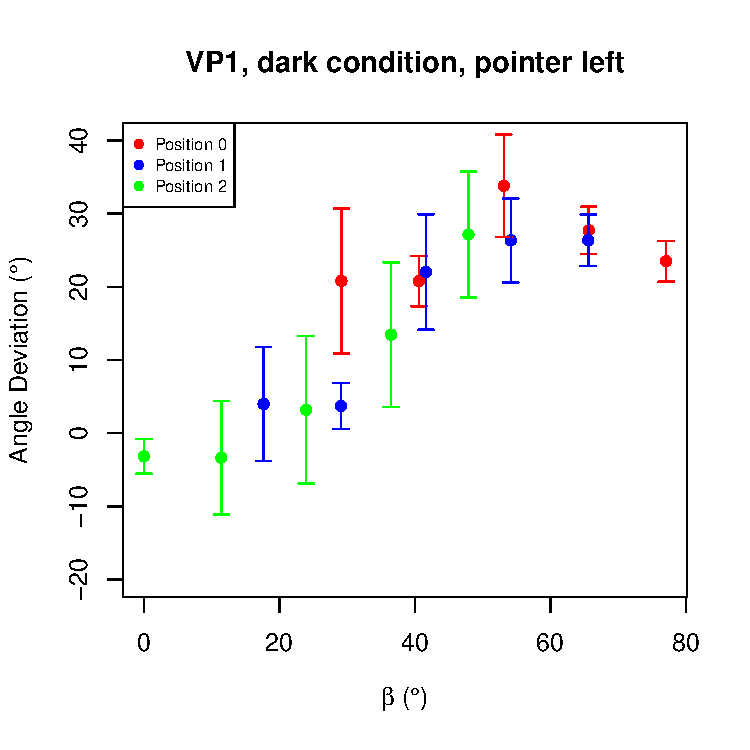
\includegraphics[width = 7cm]{Images/plots/AngleDevVP1DarkLeft.pdf}
    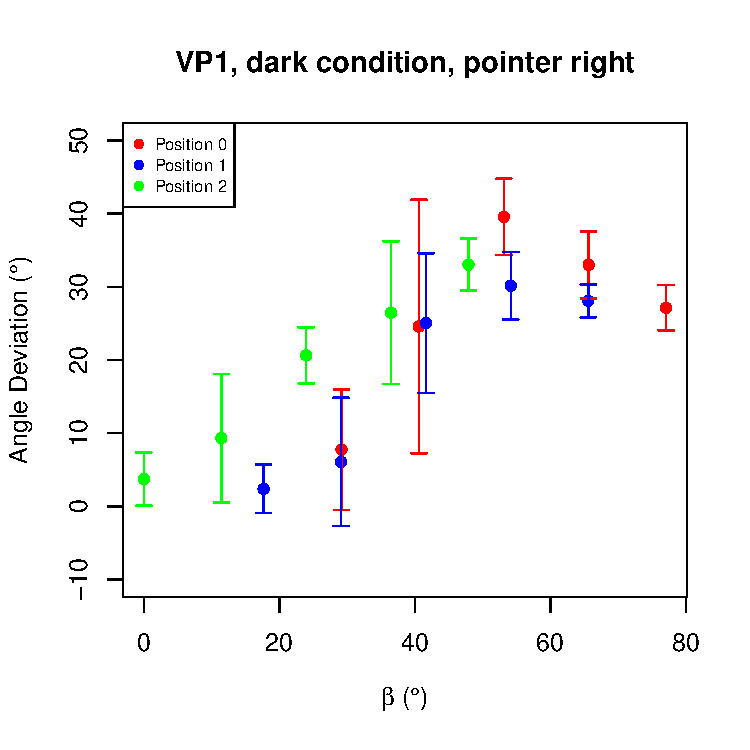
\includegraphics[width = 7cm]{Images/plots/AngleDevVP1DarkRight.pdf}
    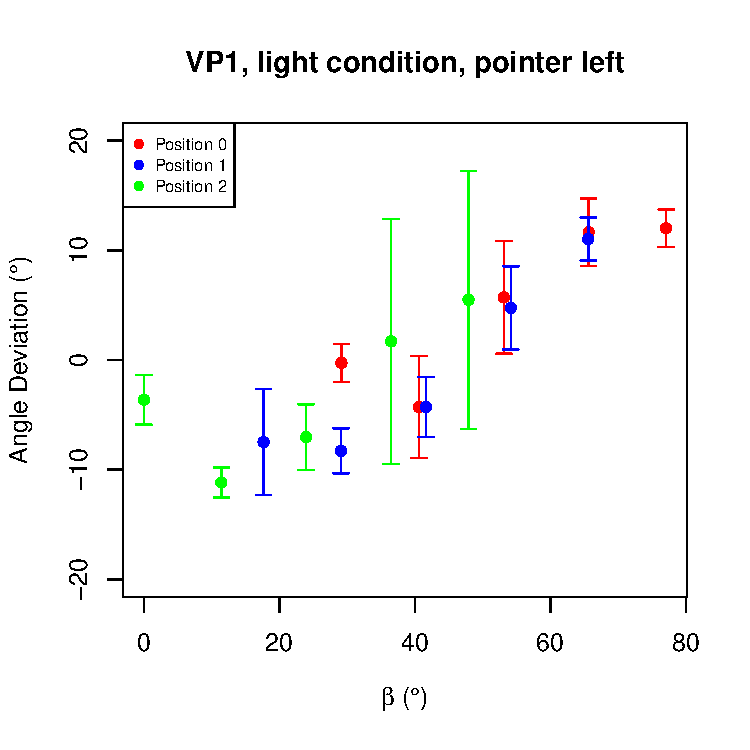
\includegraphics[width = 7cm]{Images/plots/AngleDevVP1LightLeft.pdf}
    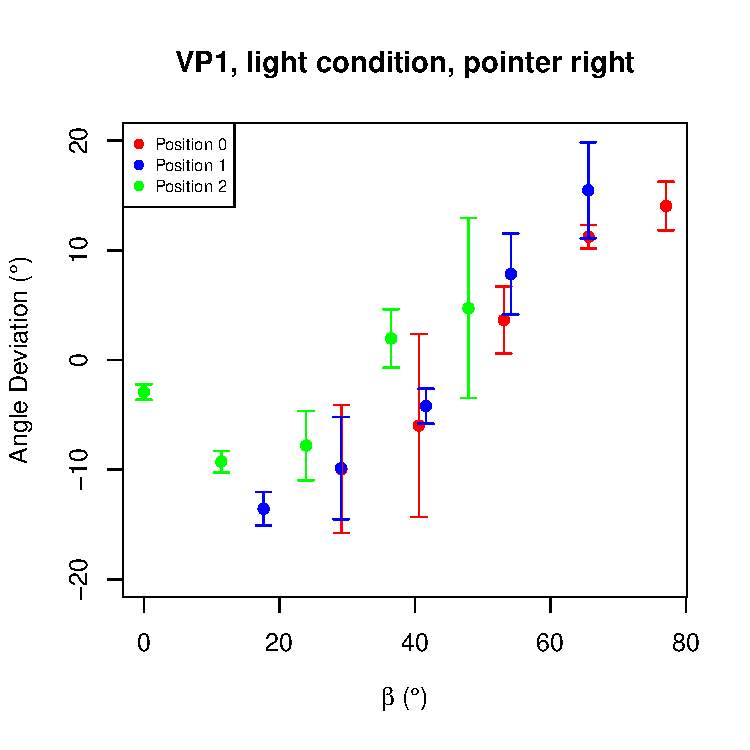
\includegraphics[width = 7cm]{Images/plots/AngleDevVP1LightRight.pdf}
    \caption{The mean angle deviation of the first subject (VP1) per pointer position and light condition (pointer left/right, lighting dark/light) for each subject position by $\beta$. Error bars indicate the standard deviation. Be aware of the partly different scale on the y-axis.} 
    \label{DeviationVP1}
\end{figure}
\begin{figure}
    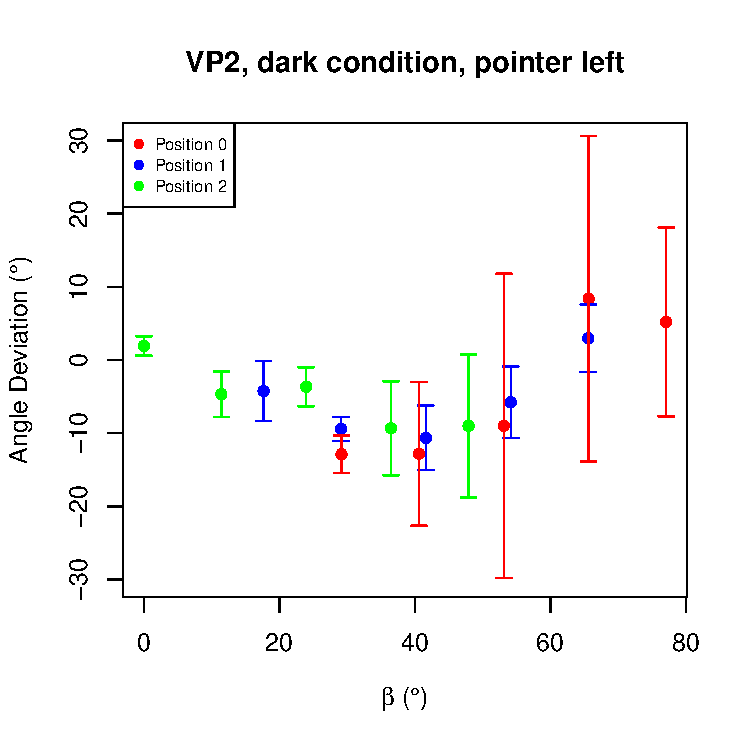
\includegraphics[width = 7cm]{Images/plots/AngleDevVP2DarkLeft.pdf}
    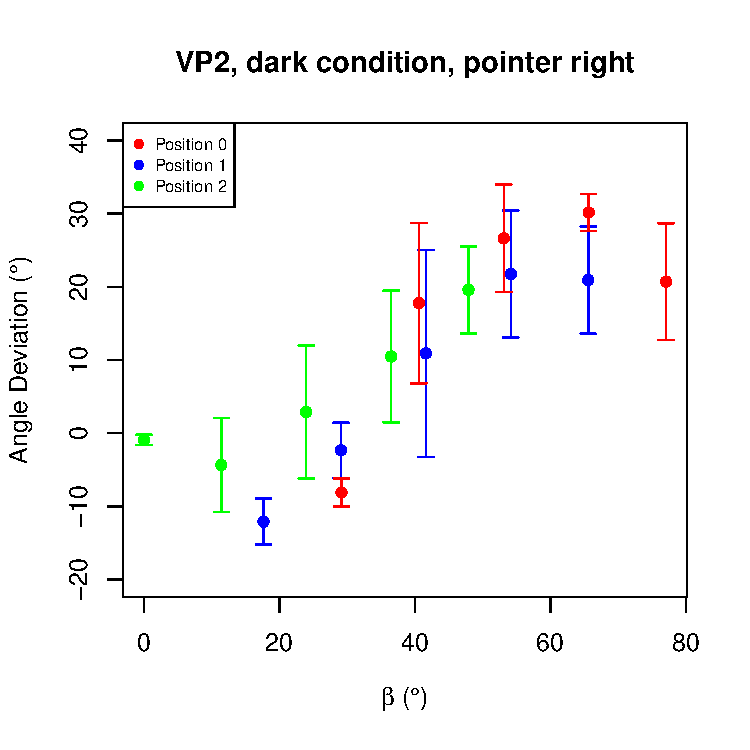
\includegraphics[width = 7cm]{Images/plots/AngleDevVP2DarkRight.pdf}
    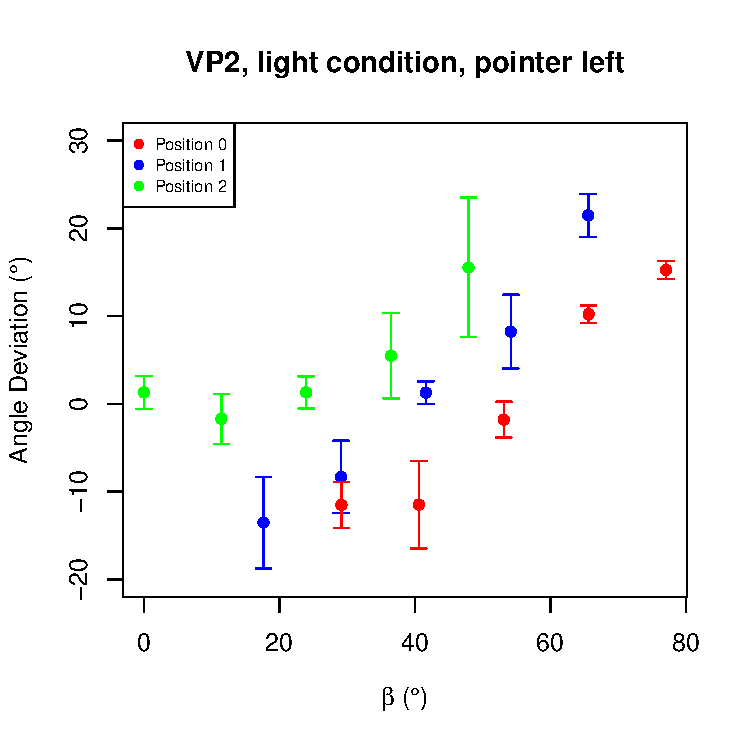
\includegraphics[width = 7cm]{Images/plots/AngleDevVP2LightLeft.pdf}
    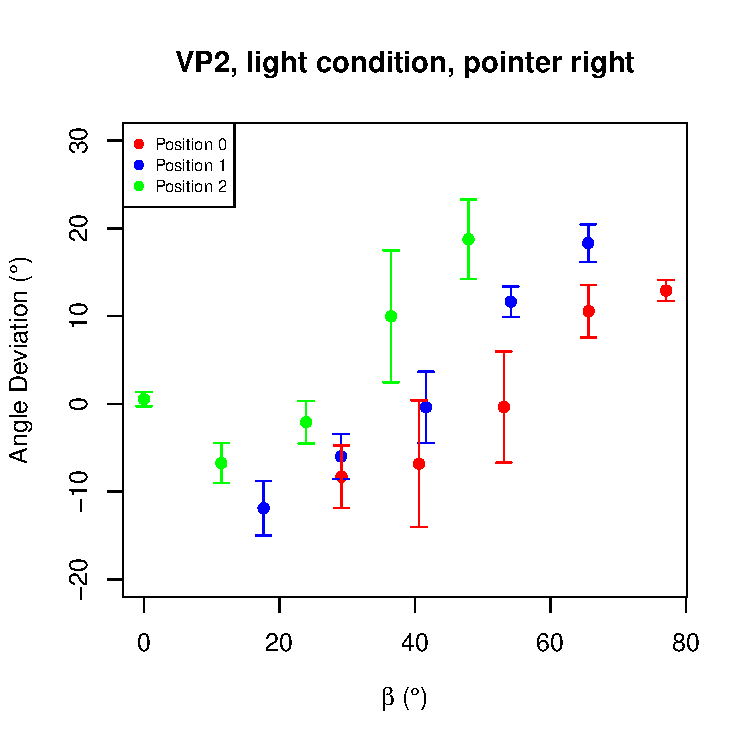
\includegraphics[width = 7cm]{Images/plots/AngleDevVP2LightRight.pdf}
    \caption{The mean angle deviation of the second subject (VP2) per pointer position and light condition (pointer left/right, lighting dark/light) for each subject position by $\beta$. Error bars indicate the standard deviation. Be aware of the partly different scale on the y-axis.} 
    \label{DeviationVP2}
    
\end{figure}
\begin{figure}
    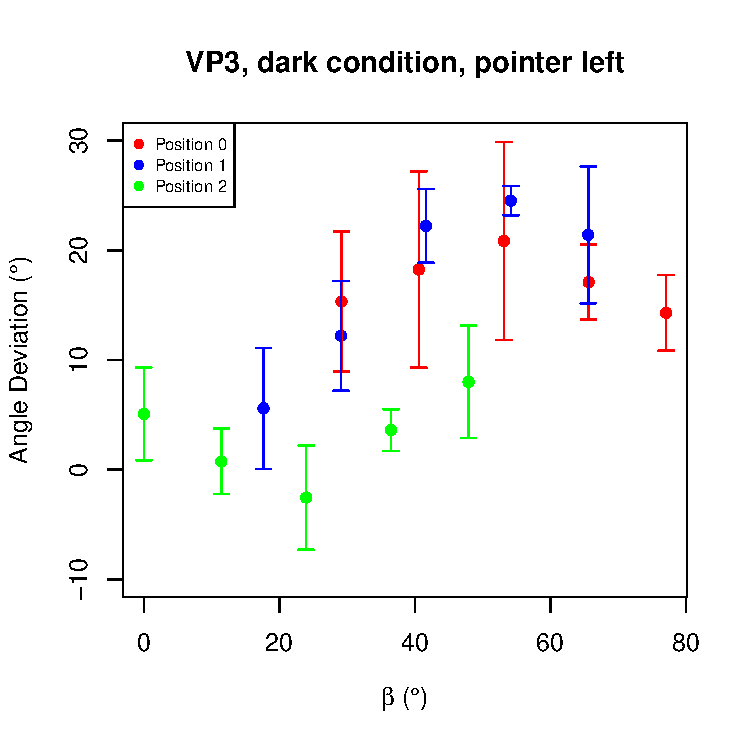
\includegraphics[width = 7cm]{Images/plots/AngleDevVP3DarkLeft.pdf}
    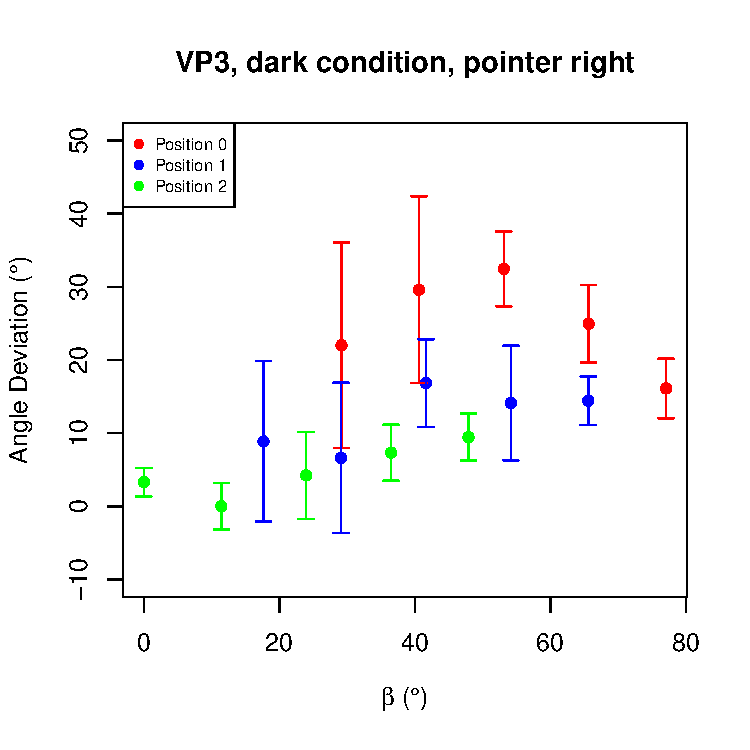
\includegraphics[width = 7cm]{Images/plots/AngleDevVP3DarkRight.pdf}
    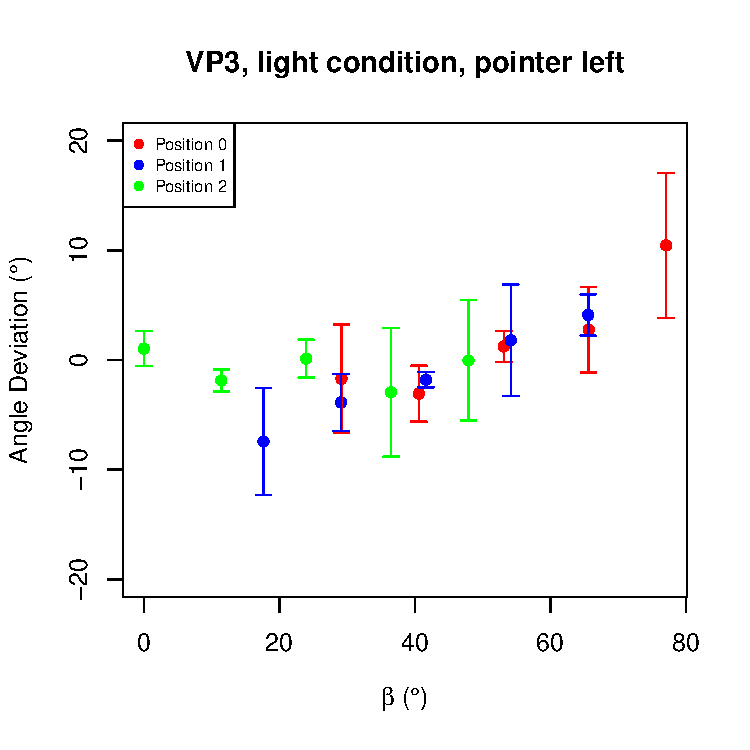
\includegraphics[width = 7cm]{Images/plots/AngleDevVP3LightLeft.pdf}
    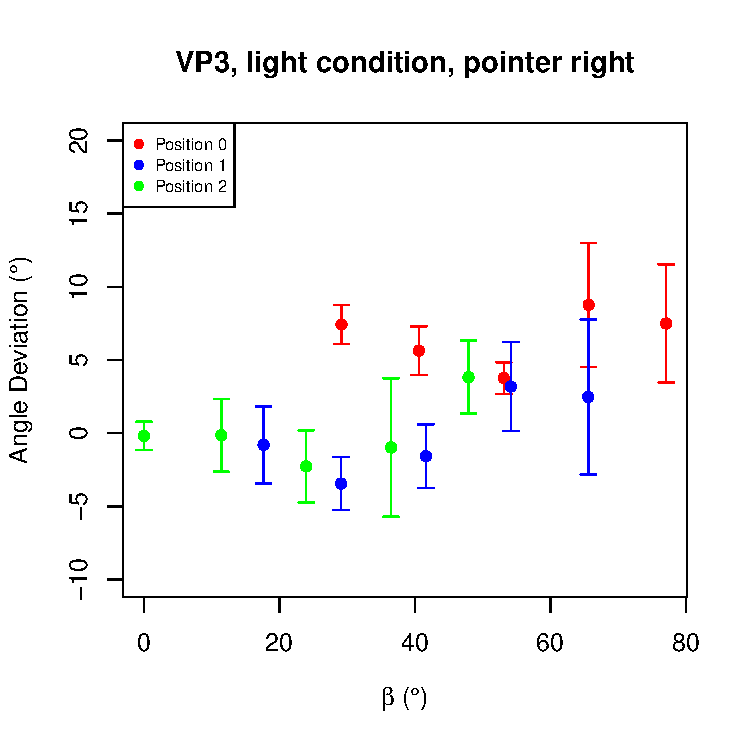
\includegraphics[width = 7cm]{Images/plots/AngleDevVP3LightRight.pdf}
    \caption{The mean angle deviation of the third subject (VP3) per pointer position and light condition (pointer left/right, lighting dark/light) for each subject position by $\beta$. Error bars indicate the standard deviation. Be aware of the partly different scale on the y-axis.} 
    \label{DeviationVP3}
\end{figure}
\begin{figure}
    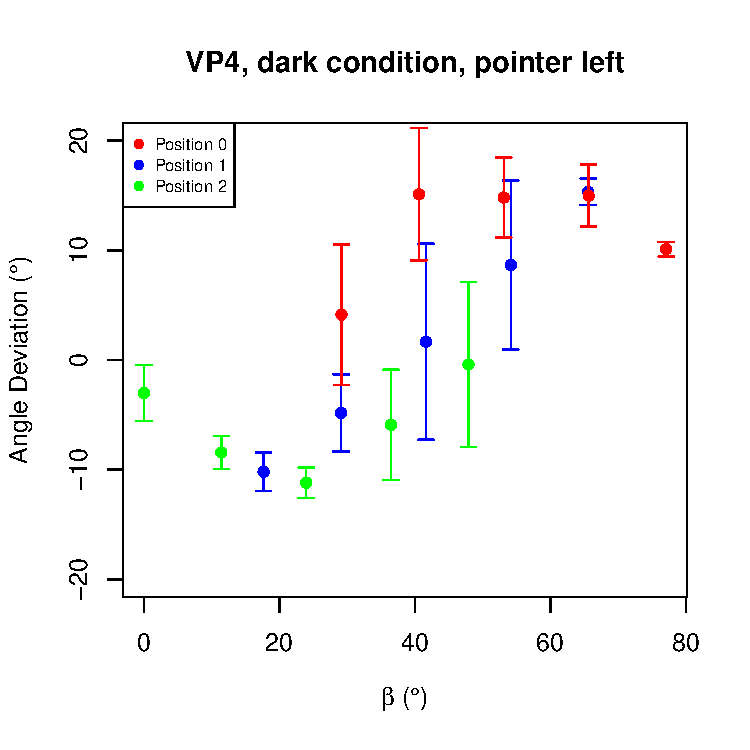
\includegraphics[width = 7cm]{Images/plots/AngleDevVP4DarkLeft.pdf}
    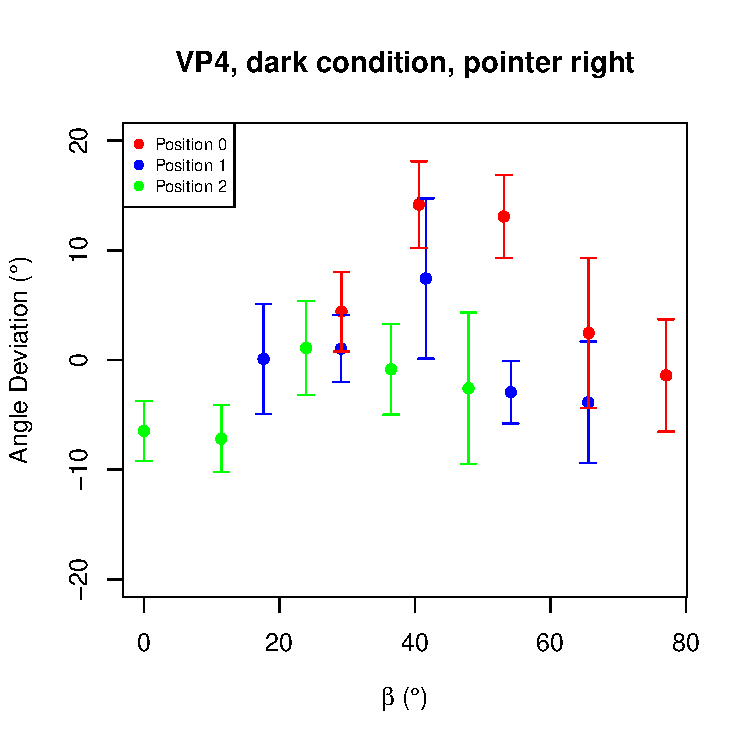
\includegraphics[width = 7cm]{Images/plots/AngleDevVP4DarkRight.pdf}
    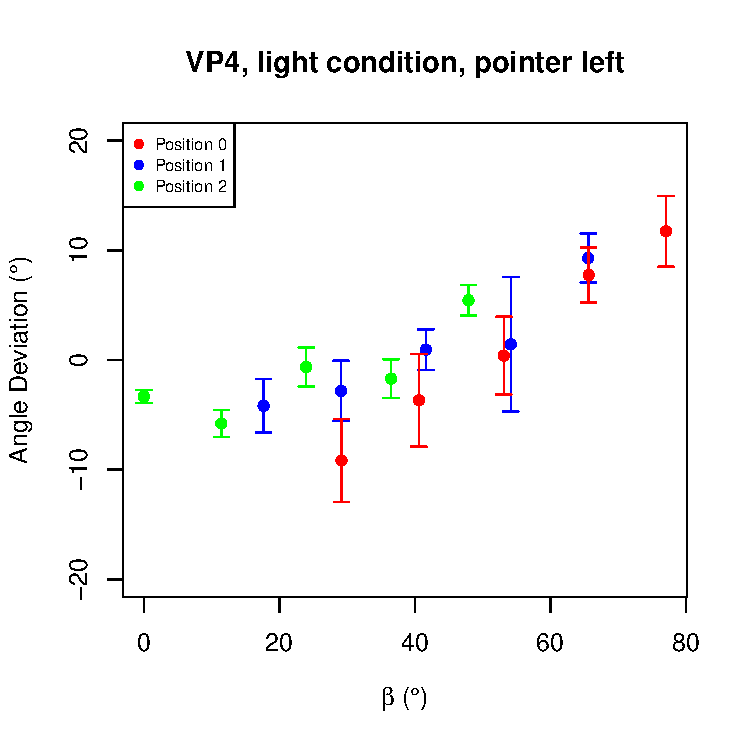
\includegraphics[width = 7cm]{Images/plots/AngleDevVP4LightLeft.pdf}
    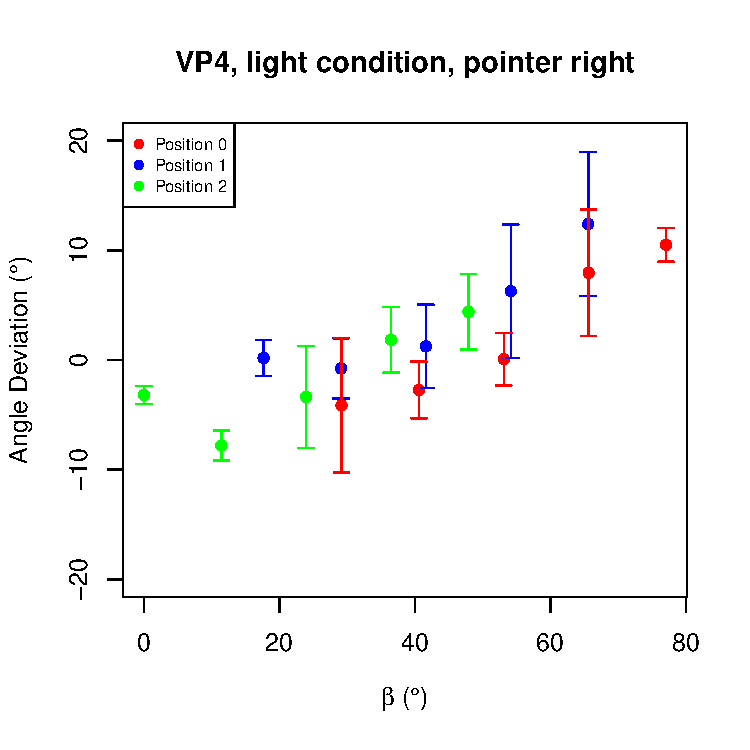
\includegraphics[width = 7cm]{Images/plots/AngleDevVP4LightRight.pdf}
    \caption{The mean angle deviation of the fourth subject (VP4) per pointer position and light condition (pointer left/right, lighting dark/light) for each subject position by $\beta$. Error bars indicate the standard deviation.} 
    \label{DeviationVP4}
\end{figure}

In figure \ref{DeviationVP2} the same is depicted for the second subject (VP2). Note that in the light condition for both symmetries the means can be distinguished with regard to the different subject positions (marked in red, green, and blue). A similar distinction of at least two subject positions can be seen in figure \ref{DeviationVP3}, showing the deviation of the third subject (VP3) in the dark condition. Also interesting is that VP3 had mainly very small deviations in the light condition. The same can be observed for the fourth subject (VP4) as seen in figure \ref{DeviationVP4}. The development of the deviation by $\beta$ for VP4 in the light condition is almost a straight, as the deviation in total is very small for most angles. 
Overall, all four subjects show a similar shape with negative deviations with a smaller $\beta$ and positive deviations as $\beta$ increases.

%beta
Deviations per conditions were compared using analyses of variance (ANOVAs) over the factors lighting, pointer position (symmetry), $\beta$, and subject position with a significance level of $p < .05$. They confirmed the observations of the graphs. For each subject the angle $\beta$ was very sig\-ni\-fi\-cant (VP1:$F(1,36) = 156.99, p < .001$, VP2:$F(1,36) = 95.87, p < .001$, VP3:$F(1,36) = 84.07), p < .001$, VP4:$F(1,36)= 95.09, p < .001$). This has been expected, having looked at the graphs, as the deviation indeed changes drastically depending on $\beta$.

%lighting
A main effect for the lighting could only be shown for VP1 and VP3, but in both cases it was very significant ($F(1,36) = 193.11, p < .001$ and $F(1,36) = 196.05, p < .001$ respectively). This is seen in figure \ref{DeviationVP1} and \ref{DeviationVP3} with a higher positive deviation for the dark condition than for the light condition.

%pointerPosition
The pointer position was very significant for VP2 ($F(1,36) = 33.68, p < .001$) and significant for VP3 $(F(1,36) = 4.95, p = .032$). That means these subjects did not show a symmetric deviation, the curvature depended on the side the pointer and the targets were placed. Figure \ref{VP2Symmetry} gives a deeper insight into the effect of the pointer position. %widerspricht meiner Kopfbewegungsidee. 
In this figure the difference of deviation (left pointer condition minus right pointer condition) by $\beta$ is depicted. It shows that for large values of $\beta$ the symmetry is not given. VP3 shows a similar but smaller effect. % should I also show the graphik for this VP

\begin{figure}
    \centering
    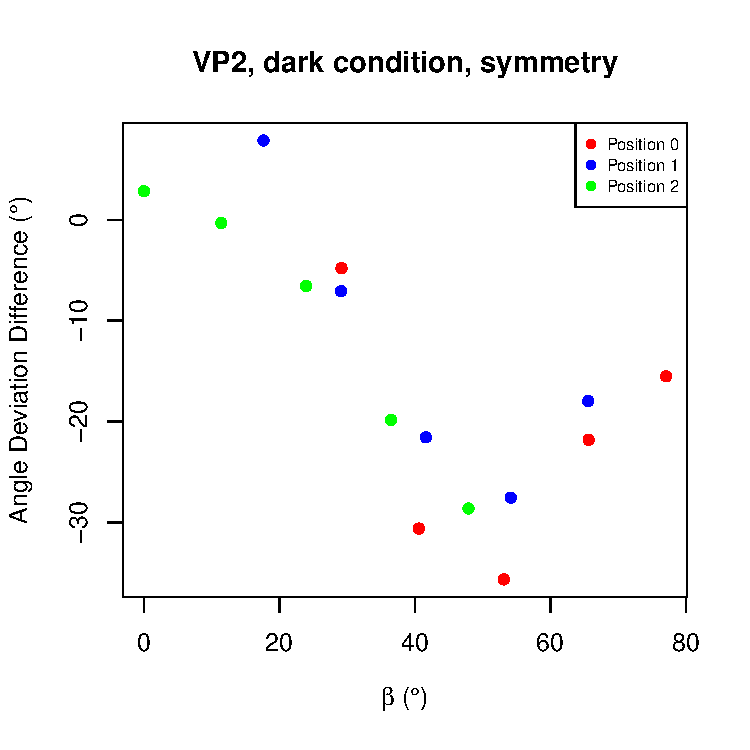
\includegraphics[width=7cm]{Images/plots/VP2Symmetry.pdf}
    \caption{The angle deviation difference (left pointer condition minus right pointer condition) for VP2 per subject position for the dark condition by $\beta$. If perfect symmetry was given, the values would be 0.}
    \label{VP2Symmetry}
\end{figure}

%subjectPosition
The position of the subject, i.e. the distance of the subject to the pointer and the targets, was very significant for VP2 and VP3 ($F(1,36) = 18.13, p < .001$ and $F(1,36) = 18.80, p < .001$ respectively), significant for VP1 ($F(1,36) = 3.49, p = .041$), and showed a tendency for VP4. For VP3 and VP4 this is clearly seen in the dark condition (figure \ref{DeviationVP3} and \ref{DeviationVP4}), for VP2 this effect can be seen in the light condition (figure \ref{DeviationVP2}) as in these graphs the different positions show different deviations for the same value of $\beta$.

This main effect of subject position cannot be set equal to the distance to the stimuli. The subject position only partly reflects the distance of the subject to the stimuli, as the distance not only depends on the subject, but also the target which is aimed at. Another representation of the deviation is in form of geodesics. It can be seen in figure \ref{VP1Curves}. The geodesics in these graphs have been approximated for each mean. The deviation was taken as the tangent for the circle arc. 
The scale of the different subject positions has been manipulated to enable the comparison of the different curves of different subject positions. Also the colour indicates the distance of the targets to the subject.  For example, target 1 in the graph of subject position 1 and target 2 in the graph of subject position 2 do have the same distance to the subject, and can hence be compared to check for the influence of the subject position. Figure \ref{VP1Curves} shows that overall the curvature is most elliptic for targets furthest away from the subject and becomes hyperbolic for targets closer to the subject. For example the red geodesic is slightly hyperbolic for all three subject positions. That means that for VP1 in the light right pointer condition a clear tendency of the influence of the subject's distance to the stimuli, i.e. not only to the pointer but also to the targets, can be seen.  

\begin{figure}
    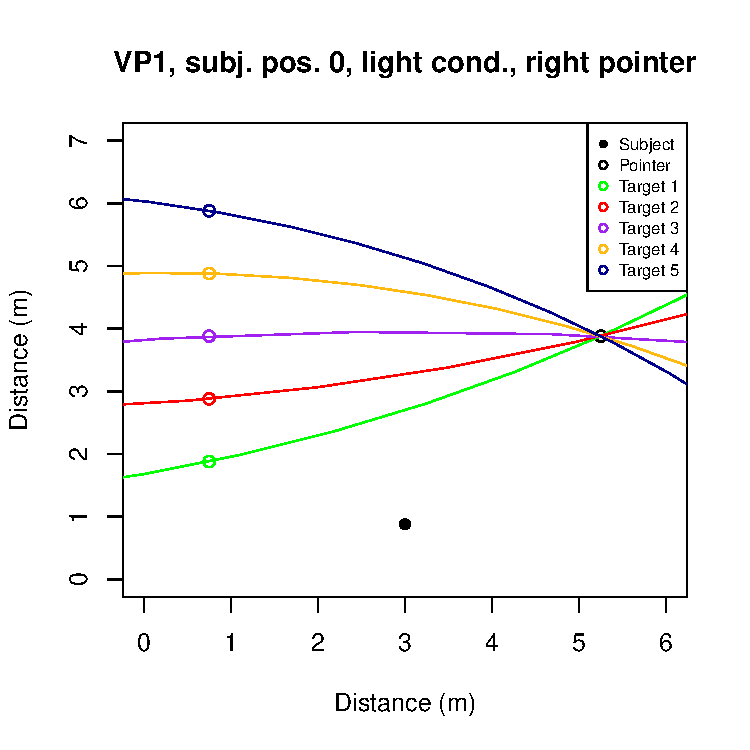
\includegraphics[clip, trim = 0.1cm 0.5cm 0.95cm 0.6cm, width=4.85cm]{Images/plots/VP1lightrightPos0Curves.pdf}
    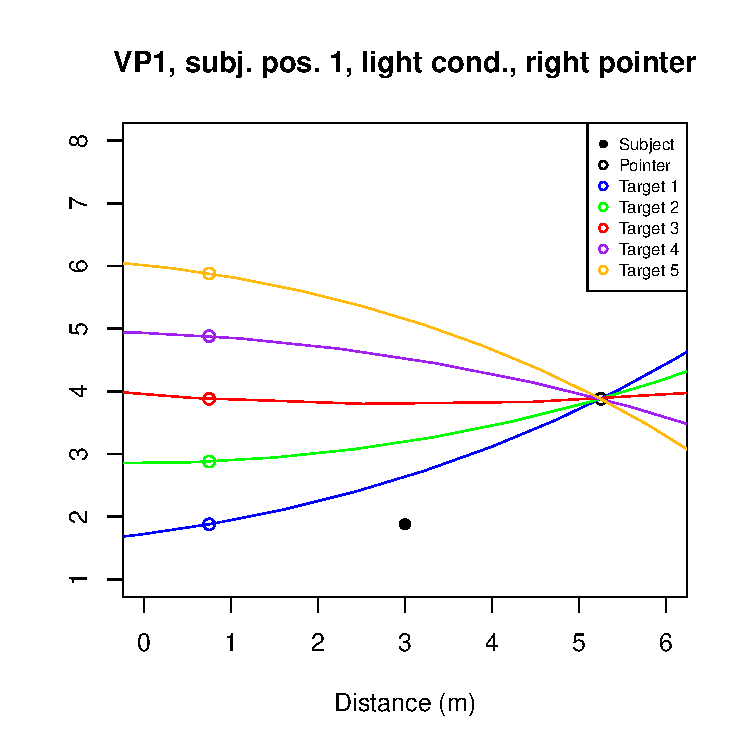
\includegraphics[clip, trim = 1.15cm 0.5cm 0.95cm 0.6cm, width=4.4cm]{Images/plots/VP1lightrightPos1Curves.pdf}
    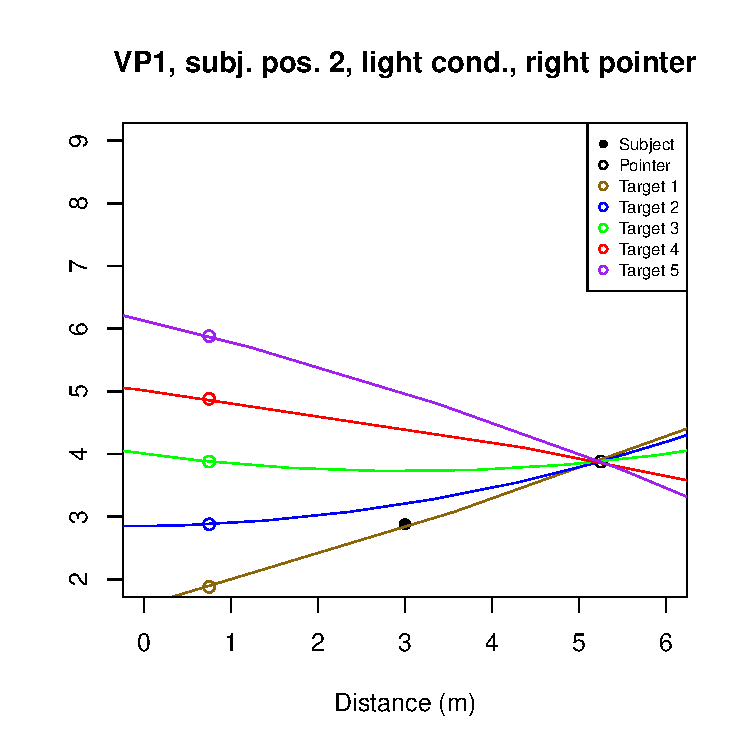
\includegraphics[clip, trim = 1.15cm 0.5cm 0.95cm 0.6cm, width=4.4cm]{Images/plots/VP1lightrightPos2Curves.pdf}
    \caption{The curvature of the intrinsic visual space approximated by geodesics for each target position for VP1 in the light, right pointer condition. The scale has been changed for each subject position to allow comparison of the curvature per distance of the subject to the targets. The colours encode for the distance of the targets to the subject. (0,0) marks the left rear corner of the room.}
    \label{VP1Curves}
\end{figure}

Additionally to these main effects, some interactions have been found. In the following only interactions between two factors will be discussed, even if some significant triple interactions have been found. Generally, interactions strongly depended on the subject, i.e. were only found significant for one or two subjects. The expected interaction between lighting and pointer position was only found to be significant for VP2 ($F(1,36) = 29.09, p < .001$) and a tendency was found for VP1. Note that VP2 was also the only subject who showed a very significant effect of pointer position. Interesting %worwahl (Augen verdrehen)
is a very significant interaction of lighting and subject position for VP2, VP3, and VP4 ($F(1,36) = 6.78, p = .032, F(1,36) = 15.21, p<.001$ and $F(1,36) =17.87, p < .001$ respectively). Also unexpected is a very significant interaction between the pointer position and the subject position for VP3 ($F(1,36) = 8.58, p<.001$) and a tendency for this interaction for VP1.
And finally for VP2 a very significant interaction ($F(1,36) = 6.83,p = .0031$), for VP3 a significant interaction ($F(1,36) = 5.12, p = .011$) and a tendency for VP1 between $\beta$ and the subject position was found. As $\beta$ directly depends on the subject position, this is not surprising. 
%sollte ich F-Werte bei Tendenzen angeben?

%Interaction pointer position and $\beta$. TODO wo erwähne ich die denn in der Diskussion?

\begin{figure}
    \centering
    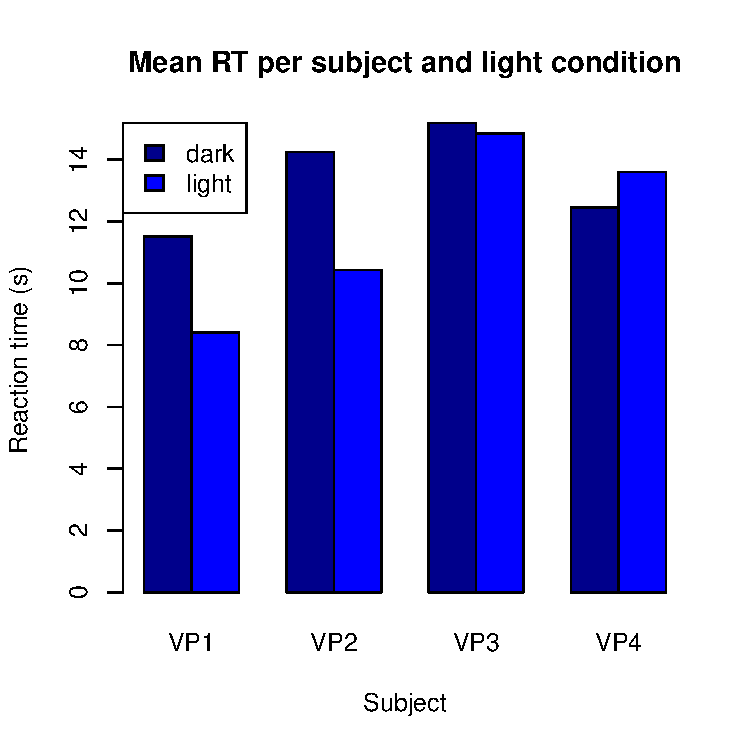
\includegraphics[width=7cm]{Images/plots/ReactionTimes.pdf}
    \caption{The mean reaction times per subject and light condition in seconds.}
    \label{ReactionTime}
\end{figure}

\section{Reaction time}
The reaction time per trial does not have a great informative value, as the time to rotate the pointer is included in the reaction time. For example, once per block the subjects pointed at target 1 right after pointing at target 5. This takes much longer than to rotate the pointer to target 1 from target 2. This results in a great variation of the reaction time values. While the mean over all subjects in seconds is $12.58$, the standard deviation is almost as high ($SD = 10.24$). Even so, the reaction time can be compared as means per condition.

The difference of the reaction time in the dark and the light condition per subject is shown in figure \ref{ReactionTime}. It shows that most subjects were faster in the light condition. This was confirmed by a two-sided paired t-test. Over all subjects the reaction time in the light condition was significantly shorter than in the dark condition ($t(478) = -2.60, p = .0097$). It is interesting to note that VP3 and VP4, who show a similar reaction time in both lighting conditions, are also those who showed only small deviations in the light condition (see figures \ref{DeviationVP3} and \ref{DeviationVP4}). 


\section{Comparison to real life experiment}
To compare this experiment to the real life experiment and hence to examine the usefulness of virtual reality for our research question, the data of the subject which participated in both experiments was compared. In figure \ref{DeviationBOTHVP5} the mean deviation by $\beta$ of this fifth subject (VP5) is shown for both the real life experiment (RL) and the virtual reality experiment (VR). The values of the two experiments can be distinguished by colour and symbol shape. In the light condition the deviation is surprisingly similar. For the left and the right pointer condition especially the deviations on subject position 2 are almost identical, the means of which can be distinguished from the other subject positions. In the dark condition in the pointer right condition a similar overlap can be seen, while on the other hand in the pointer left conditions great discrepancies are visible. In this condition in VR the deviation has relative smaller values for $\beta$ greater than 20\textdegree{} than in RL. Particularly interesting is that, while the deviations of subject position 0 remain fairly similar, the deviations of subject position 1 and 2 are very different. Overall, VP5 provided similar deviations in both experiments.
% Discussion: leading to the conclusion, that VR is indeed a possible measurement for the intrinsic geometry of the visual space. %Discussion?


\begin{figure}
    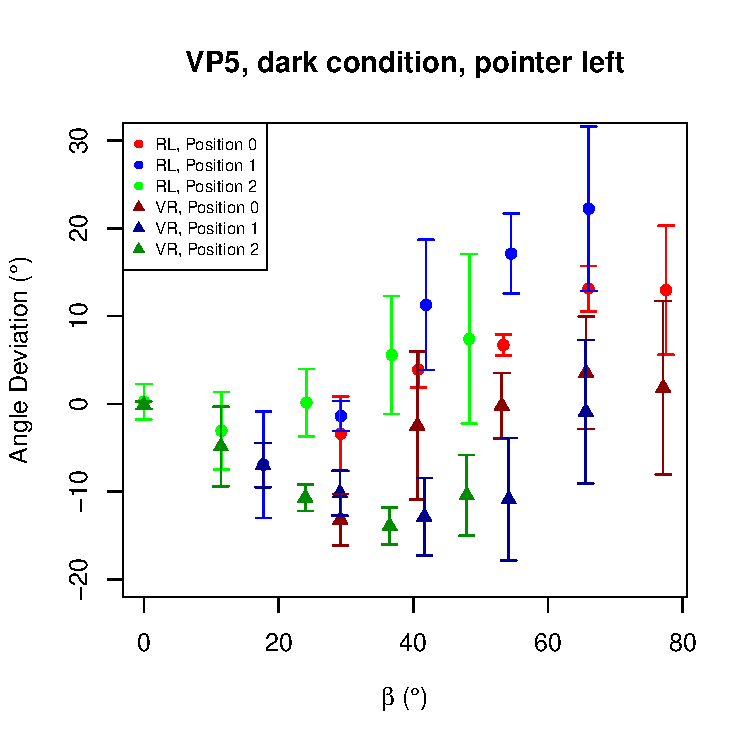
\includegraphics[width = 7cm]{Images/plots/AngleDevVP5BOTHDarkLeft.pdf}
    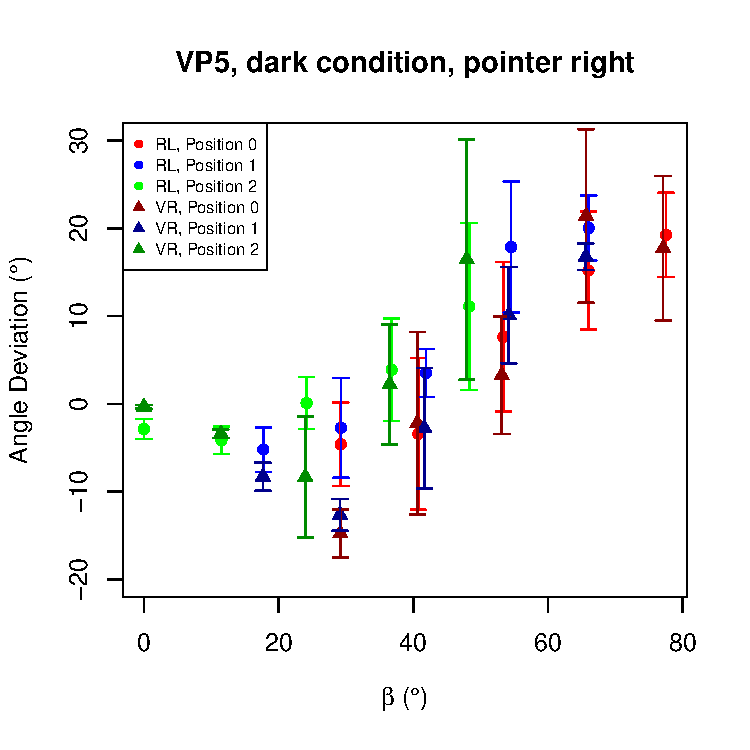
\includegraphics[width = 7cm]{Images/plots/AngleDevVP5BOTHDarkRight.pdf}
    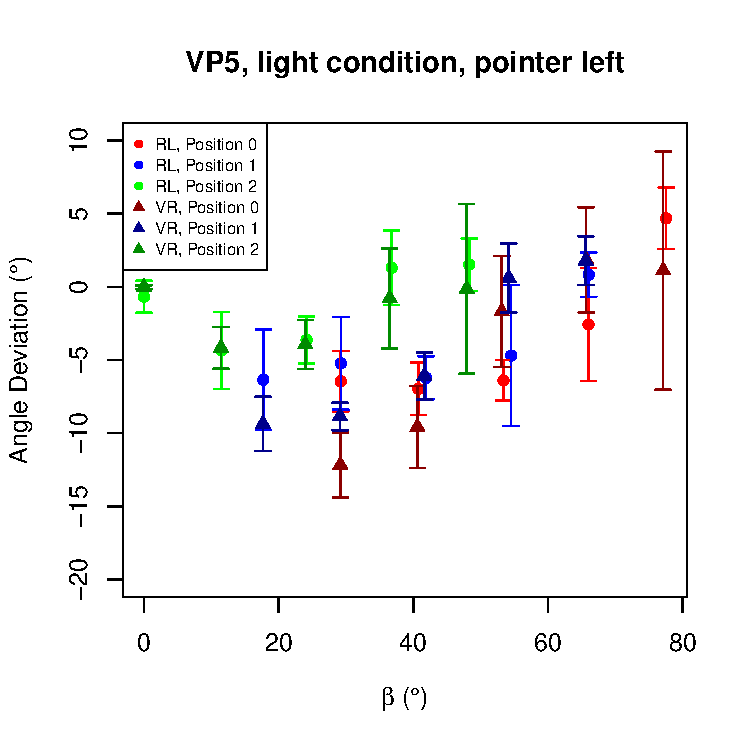
\includegraphics[width = 7cm]{Images/plots/AngleDevVP5BOTHLightLeft.pdf}
    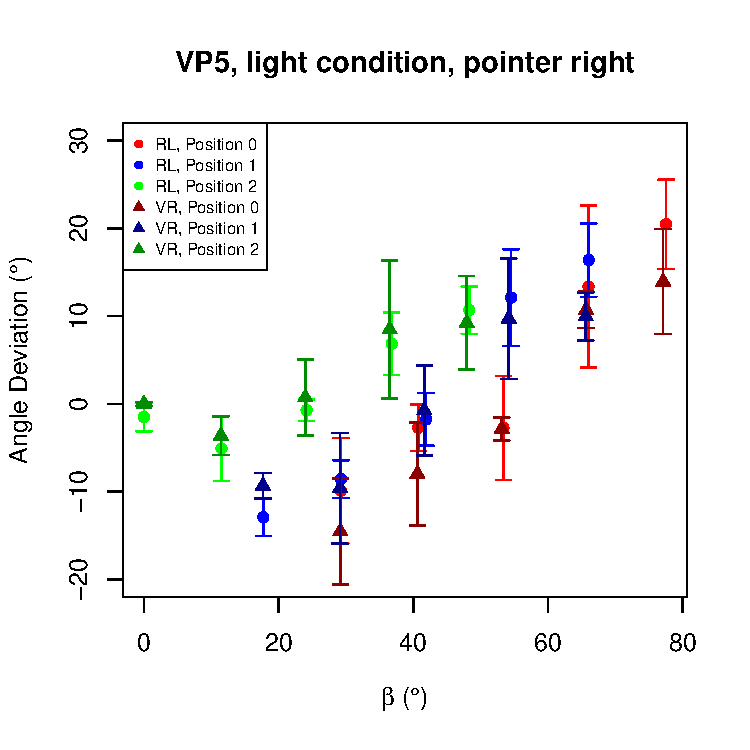
\includegraphics[width = 7cm]{Images/plots/AngleDevVP5BOTHLightRight.pdf}
    \caption{The mean angle deviation of the fifth subject (VP5) per pointer position and light condition (pointer left/right, lighting dark/light) for each subject position by $\beta$ for both the real life experiment (RL) and the virtual reality experiment (VR). Error bars indicate the standard deviation. Be aware of the partly different scale on the y-axis.} 
    \label{DeviationBOTHVP5}
\end{figure}


%For this purpose one of the subjects participated in the real life experiment, will also take part in this experiment. Obviously this subject cannot be counted as naive subjects, but as the curvature of the visual space varies per person, hence comparison of data of different subjects is difficult, this may be the best possibility to compare the impact of doing the task in virtual reality in contrast of doing it in real life. 

% HeadMovement?






% values of beta instead of angles of beta.

%always say point instead of aim

%hier falsche wortwahl mit positive and negative curvature, instead elliptic and hyperbolic

%nai\"{}ve